\section{Results}
\label{sec:results}

Table~\ref{tab:cross-run} consolidates the nine-run sequence under the
EXP-004 proxy. Figure~\ref{fig:cross-backbone-gradient} visualises the
pretraining-data gradient. Per-run plots --- pair-score histograms,
training-loss trajectories, and representation-health values --- live in the
run archive at \runarchive\ under each run's \texttt{<run\_id>/} folder; the
appendix reproduces the most relevant cross-run summary tables.

% Table 1: cross-run results on the EXP-004 proxy.
% Source: paper/figures/locked-numbers.json (verified by paper/verify_claims.py).
\begin{table}[h]
\centering
\small
\setlength{\tabcolsep}{4pt}
\begin{tabular}{@{}llllrrr@{}}
\toprule
Run & Backbone & Predictor & Opt. & Train $\auroc$ & Test $\auroc$ & $\Delta$ \\
\midrule
EXP-001  & DINOv2 ViT-B/14    & linear  & SGD  & $1.000$ & $1.000$            & $0.000$ \\
EXP-002  & DINOv2 ViT-B/14    & linear  & SGD  & $0.953$ & $0.920$            & $+0.269$ \\
EXP-003  & DINOv2 ViT-B/14    & linear  & SGD  & $0.953$ & $0.680$            & $-0.281$ \\
EXP-004  & DINOv2 ViT-B/14    & linear  & SGD  & $0.900$ & $0.249$            & $-0.331$ \\
EXP-005  & DINOv2 ViT-B/14    & MLP     & SGD  & $0.572$ & $0.270$            & $-0.310$ \\
EXP-006a & DINOv2 ViT-B/14    & MLP     & Adam & $0.893$ & $0.248$            & $-0.332$ \\
EXP-006b & OpenAI CLIP B/16   & linear  & SGD  & $0.986$ & $0.286$            & $-0.294$ \\
EXP-008  & BiomedCLIP B/16    & linear  & SGD  & $0.912$\textsuperscript{\dag} & $\mathbf{0.329 \pm 0.012}$\textsuperscript{\ddag} & $-0.252$ \\
EXP-007  & DermLIP B/16\textsuperscript{$\star$}    & linear  & SGD  & $1.000$ & $\mathbf{0.944 \pm 0.003}$\textsuperscript{\ddag} & $\mathbf{+0.363}$ \\
\bottomrule
\end{tabular}
\caption{Cross-run results on the EXP-004 proxy (HAM10000,
leakage-controlled splits, $1{,}000$ stable $+$ $1{,}000$ changing pairs
per split). Test column is $\auroc$ on \strongholdtwo; $\Delta$ is
versus the strongest cheap baseline on each split (pixel L2 $= 0.580$
for EXP-004 onward; SSIM or DINOv2-S cosine in earlier runs).
\textsuperscript{\dag} Seed-mean of the BiomedCLIP train $\auroc$ across
five seeds. \textsuperscript{\ddag} Mean $\pm$ sd across five seeds.
\textsuperscript{$\star$} Derm1M almost certainly contains HAM10000 raw
images; the resulting positive cannot be attributed to dermoscopy-domain
transfer with the experiments reported here (\S\ref{sec:followup}).}
\label{tab:cross-run}
\end{table}


\begin{figure}[h]
\centering
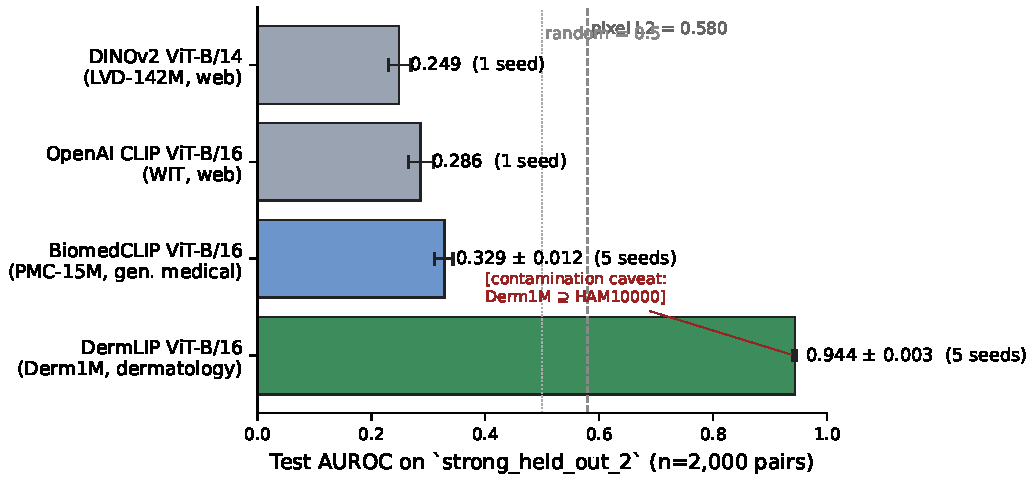
\includegraphics[width=0.85\linewidth]{figures/fig1-cross-backbone-gradient.pdf}
\caption{Test $\auroc$ on \strongholdtwo\ (the unseen third nuisance family)
under the EXP-004 recipe, across four backbones. Error bars are bootstrap
$95\%$ CIs (single seed) or seed-mean $\pm$ standard deviation across five
seeds where available. Pixel L2 (the strongest cheap baseline at $0.580$) is
shown as a dashed reference line. The DermLIP bar carries the contamination
caveat: HAM10000 image-level overlap in Derm1M cannot be excluded
(Appendix~\ref{app:contamination}), and the experiments reported here cannot
separate dermoscopy-domain transfer from such overlap (\S\ref{sec:followup}).}
\label{fig:cross-backbone-gradient}
\end{figure}

Table~\ref{tab:predictor-optimiser} isolates the predictor $\times$
optimiser axis under frozen DINOv2 ViT-B/14: across linear and MLP
predictors, under SGD and Adam, with train $\auroc$ ranging from
$0.572$ to $0.900$, test $\auroc$ on \strongholdtwo\ stays in
$[0.248, 0.270]$ (a $\pm 0.011$ half-range around the midpoint
$0.259$). Scaffold capacity is not the bottleneck.

% Table 2: predictor x optimiser ablation on the EXP-004 proxy under frozen DINOv2 ViT-B/14.
% Source: locked-numbers.json runs exp004_dinov2_linear, exp005_dinov2_mlp_sgd, exp006a_dinov2_mlp_adam.
\begin{table}[h]
\centering
\small
\setlength{\tabcolsep}{6pt}
\begin{tabular}{@{}llrrrr@{}}
\toprule
Run & Predictor & Optimiser & Train $\auroc$ & Test $\auroc$ & 95\% CI \\
\midrule
EXP-004  & linear (identity warm-start)        & SGD  & $0.900$ & $0.249$ & $[0.230, 0.270]$ \\
EXP-005  & 2-layer ID-residual MLP (under-fit) & SGD  & $0.572$ & $0.270$ & $[0.249, 0.293]$ \\
EXP-006a & 2-layer ID-residual MLP (fit)       & Adam & $0.893$ & $0.248$ & $[0.228, 0.269]$ \\
\bottomrule
\end{tabular}
\caption{Predictor $\times$ optimiser ablation under frozen DINOv2
ViT-B/14 on the EXP-004 proxy. Across two predictor classes (linear vs
MLP) and two optimisers (SGD vs Adam), train $\auroc$ ranges from
$0.572$ (under-fit MLP) to $0.900$ (linear) but test $\auroc$ on
\strongholdtwo\ stays in a $\pm 0.011$ band around $0.255$. Scaffold
capacity does not move the held-out-family floor.}
\label{tab:predictor-optimiser}
\end{table}


Table~\ref{tab:seed-sweep} reports the seed sweep on the two
contamination-relevant configurations. Both headline numbers are
seed-stable; the partition gradient is robust to seed variance.

% Table 3: seed sweep on EXP-007 (DermLIP) and EXP-008 (BiomedCLIP).
% Source: docs/experiments/EXP-007-008-seed-sweep-summary.md sections 2--4.
\begin{table}[h]
\centering
\small
\setlength{\tabcolsep}{5pt}
\begin{tabular}{@{}llcrcc@{}}
\toprule
Run & Backbone & $n$ seeds & Test $\auroc$ (mean $\pm$ sd) & Range & 95\% CI[mean] \\
\midrule
EXP-007 & DermLIP B/16    & $5$ & $0.9435 \pm 0.0029$ & $[0.939, 0.947]$ & $[0.941, 0.946]$ \\
EXP-008 & BiomedCLIP B/16 & $5$ & $0.3286 \pm 0.0120$ & $[0.312, 0.344]$ & $[0.318, 0.339]$ \\
\bottomrule
\end{tabular}
\caption{Seed sweep on EXP-007 and EXP-008. Five seeds per
configuration. Both headlines are seed-stable; the seed-mean
pretraining-data gradient (web $0.286 <$ general-medical $0.329 <$
dermoscopy $0.944$) survives. The $\sim$$4\times$ ratio between the two
seed standard deviations is consistent with the high-$\auroc$ DermLIP
regime saturating predictor parameters more reproducibly than the
partial-fit BiomedCLIP regime.}
\label{tab:seed-sweep}
\end{table}


Figure~\ref{fig:train-vs-test-scatter} plots train versus test $\auroc$
for each primary-tier run. The DINOv2 and CLIP runs cluster in the
top-right / bottom-right region (high train, low test) --- a sharp
generalisation gap. EXP-005 sits low on both axes (the under-fit MLP
that barely departed from identity). The DermLIP point is the only one
on the diagonal; BiomedCLIP fits training but does not transfer.

\begin{figure}[h]
\centering
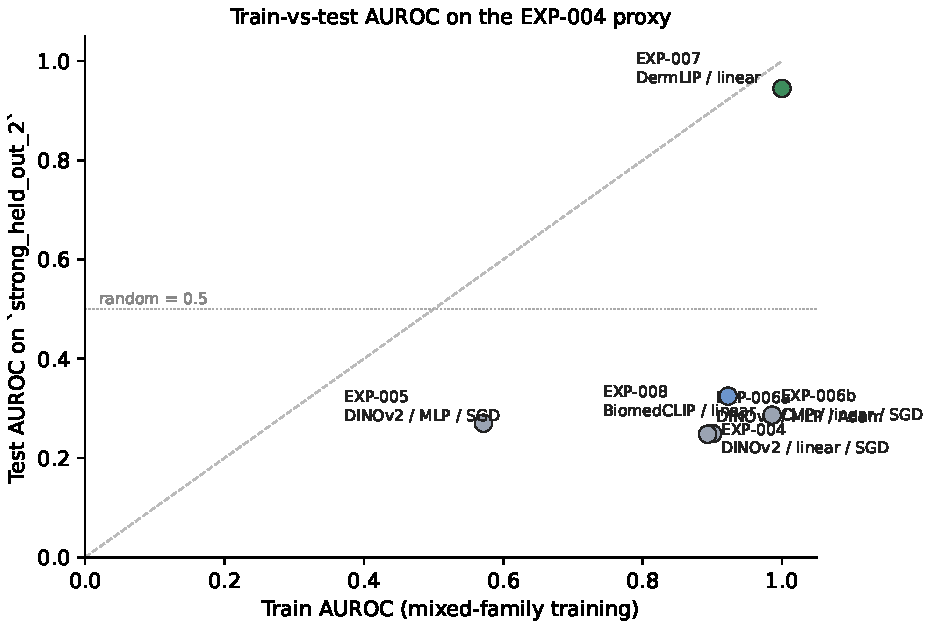
\includegraphics[width=0.78\linewidth]{figures/fig2-train-vs-test-scatter.pdf}
\caption{Train versus test $\auroc$ for each primary-tier run on the
EXP-004 proxy. The dashed diagonal is $\mathrm{train} = \mathrm{test}$;
the dotted horizontal is the random baseline at $0.5$. DermLIP is the
only configuration whose test $\auroc$ tracks training; the four
natural-image configurations sit in the inverted band below the random
line.}
\label{fig:train-vs-test-scatter}
\end{figure}

Figure~\ref{fig:pair-score-histograms} shows the test-split pair-score
distributions for the three CLIP-architecture backbones. The
predictor's score is the cosine distance between its predicted target
and the observed target, so a correctly oriented predictor places
\emph{stable}-pair scores below \emph{changing}-pair scores. CLIP and
BiomedCLIP exhibit the inverted ordering --- stable mean above changing
mean by $0.049$ and $0.034$ respectively --- while DermLIP separates
them by $+0.111$ in the correct direction. The structural inversion
visible here is the mechanism that holds test $\auroc$ to
$0.25$--$0.33$ across natural-image and general-medical pretraining
rather than at chance.

\begin{figure}[h]
\centering
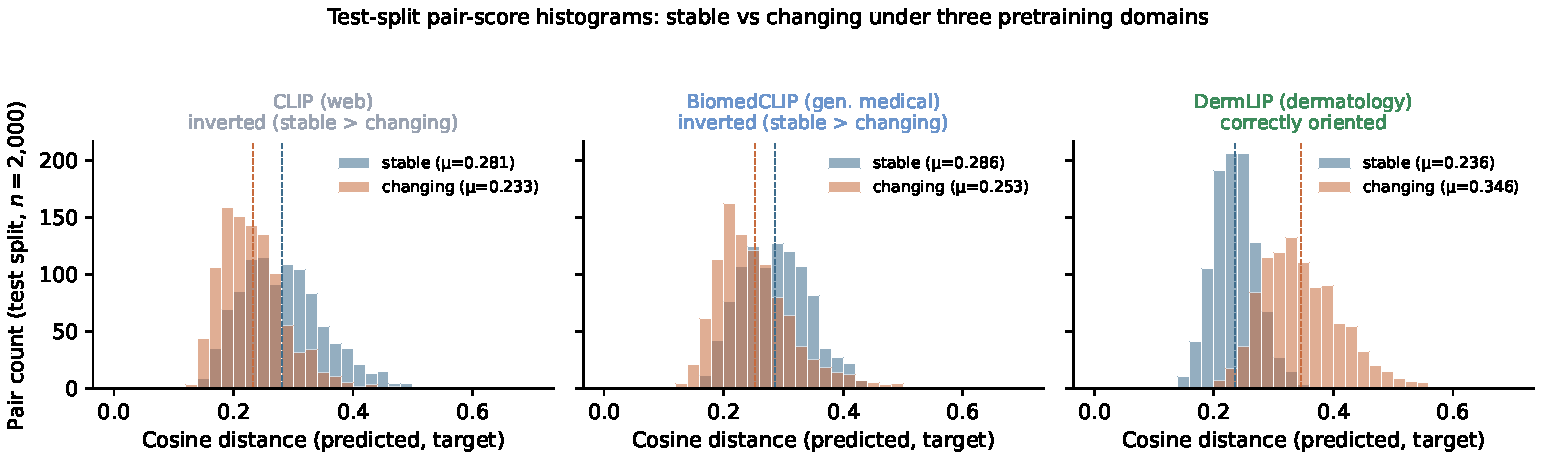
\includegraphics[width=0.98\linewidth]{figures/fig3-pair-score-histograms.pdf}
\caption{Test-split pair-score histograms (cosine distance between the
predictor's predicted target and the observed target) under three
pretraining-data domains, holding architecture (ViT-B/16) and predictor
(linear) constant. Vertical dashed lines mark per-class means. Stable
pairs should lie below changing pairs; the CLIP and BiomedCLIP panels
show the inversion that pulls test $\auroc$ below random, while the
DermLIP panel separates the two classes by $+0.111$ in the correct
direction.}
\label{fig:pair-score-histograms}
\end{figure}
